\documentclass{article}%
\usepackage[T1]{fontenc}%
\usepackage[utf8]{inputenc}%
\usepackage{lmodern}%
\usepackage{textcomp}%
\usepackage{lastpage}%
\usepackage[head=40pt,margin=0.5in,bottom=0.6in]{geometry}%
\usepackage{graphicx}%
%
\title{\textbf{Rocío San Miguel: Consejos comunales "escogerán" pacientes del buque chino}}%
\author{El Nacional Web}%
\date{22/09/2018}%
%
\begin{document}%
\normalsize%
\maketitle%
\textbf{URL: }%
http://www.el{-}nacional.com/noticias/politica/rocio{-}san{-}miguel{-}consejos{-}comunales{-}escogeran{-}pacientes{-}del{-}buque{-}chino\_252875\newline%
%
\textbf{Periodico: }%
EN, %
ID: %
252875, %
Seccion: %
Política\newline%
%
\textbf{Palabras Claves: }%
Política, Salud, Crisis humanitaria\newline%
%
\textbf{Derecho: }%
2.1, %
Otros Derechos: %
, %
Sub Derechos: %
2.1.1\newline%
%
\textbf{EP: }%
NO\newline%
\newline%
%
\textbf{\textit{Vladimir Padrino López, ministro de Defensa, aseguró que no habrá discriminación en la atención médica brindada por el buque}}%
\newline%
\newline%
%
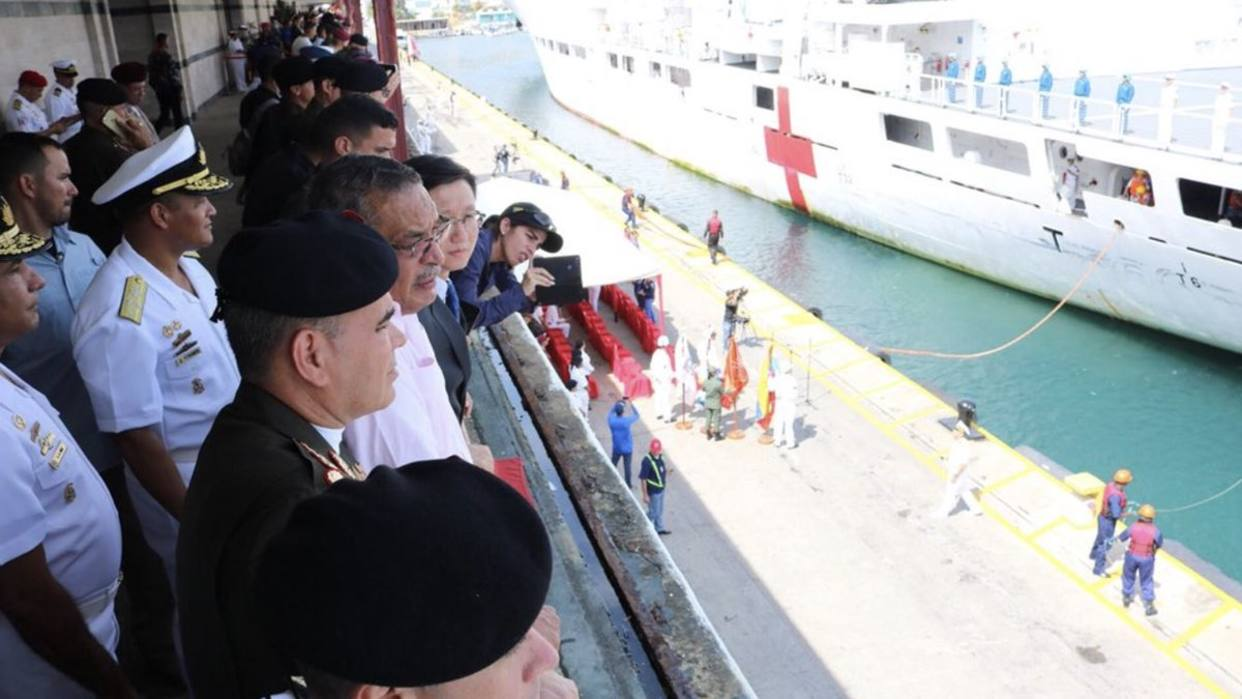
\includegraphics[width=300px]{7.jpg}%
\newline%
%
Rocío San Miguel, abogada y defensora de Derechos Humanos, denunció este sábado que los consejos comunales "escogerán" a los pacientes que recibirán atención médica por parte del buque hospital chino "Arca de la Paz".%
\newline%
%
“Llega Buque Militar Sanitario Chino. Lamentable que la atención sanitaria que darán a los venezolanos, solo puedan realizarla por conducto de los consejos comunales, quienes “escogerán” los pacientes puntuales . Segregación en la ayuda humanitaria”, indicó la abogada en Twitter.%
\newline%
%
Vladimir Padrino López, ministro de Defensa, aseguró que no habrá discriminación en la atención médica brindada por el buque, que ya recorrió más de 40 países.%
\newline%
%
"Hay 1.200 colombianos que van a tratarse, es decir, no hay discriminación alguna", declaró el funcionario de gobierno cuando arribó el buque la mañana de este sábado.%
\newline%
%
\end{document}